% !TEX root = ../thesis.tex

\chapter{Virtual Private Network -- VPN}\label{1}
Virtuálna privátna sieť (ďalej \textbf{\acrshort{vpn}}) je jeden zo spôsobov prepojenia zariadení, tak že internetová komunikácia medzi nimi je privátna, resp. zabezpečená aj v prípade používania nezabezpečenej, verejnej siete. Bezpečnosť spojenia je docielená pomocou kryptografických protokolov v tuneli, ktorý VPN vytvára. Pod pojmom tunel sa v skutočnosti myslí virtuálna zašifrovaná linka, ktorou je dátový paket prenášaný po sieti medzi koncovými zariadeniami. V skutočnosti tunel vzniká pomocou procesu zapuzdrenia dát. V závislosti od toho na akej úrovni OSI referenčného modelu sa pohybujeme. 
Táto technológia patrí aktuálne k najpoužívanejším spôsobom pripojenia sa medzi 2 rôznymi internetovými doménami. Najčastejší výskyt je možné sledovať v korporačnom prostredí, pričom cieľom je rozšírenie možností bezpečného pripojenia sa k firemnej sieti. Vzhľadom na firemné tajomstvá je nutné aby bolo takéto spojenie bezpečné a zamestnanci sa mohli pripojiť z rôznych miest. Vďaka uvedeným vlastnostiam je následne možná aj práca z~domu (z~ang. \textit{Home office}), ktorá môže byť benefitom pre obe strany. Ukážka použitia VPN je znázornená pomocou \ref{vpndemo} a \ref{vpnfancy}. 

\begin{figure}[!h]
	\centering
	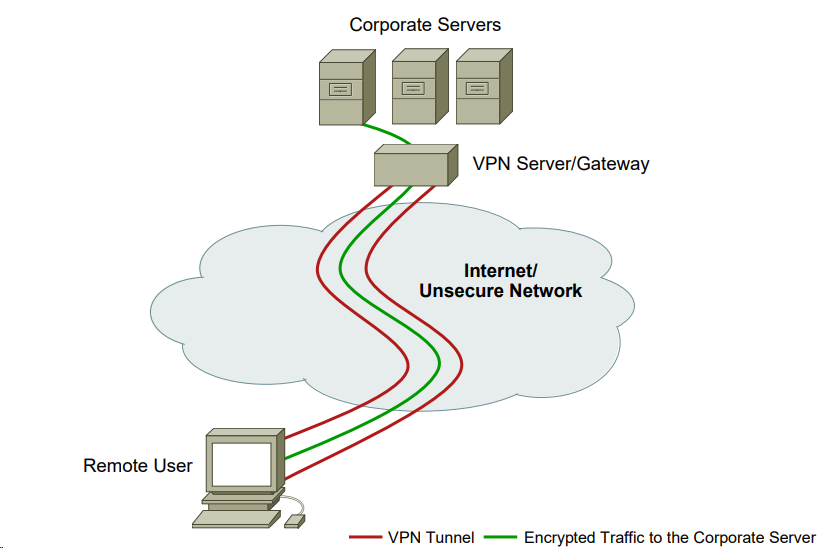
\includegraphics[width=.8\textwidth]{figures/VPNdemo}
	\caption{Ukážka typického VPN pripojenia}
	\label{vpndemo}
\end{figure}
% TODO: \usepackage{graphicx} required
\begin{figure}
	\centering
	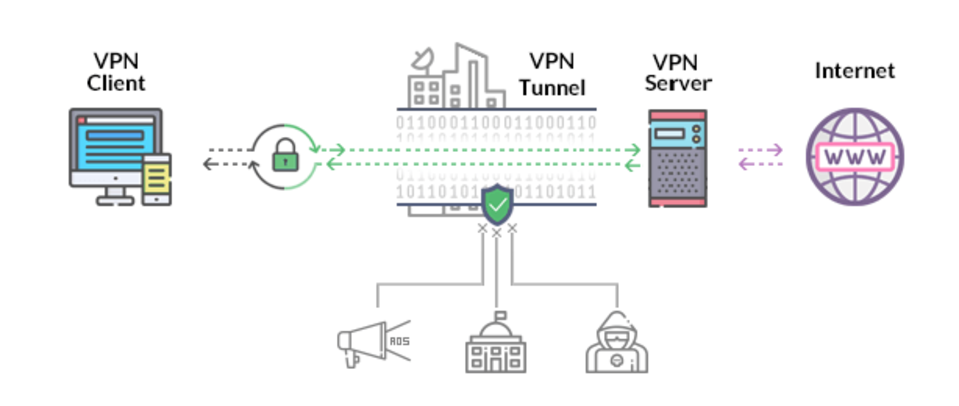
\includegraphics[width=0.7\linewidth]{figures/vpn_fancy}
	\caption{vpn fancy obrazok}
	\label{vpnfancy}
\end{figure}

https://www.webhostingsecretrevealed.net/blog/security/how-vpn-works/

\section{Výhody a nevýhody VPN sieti}
neviem ci to bude rozsahovo treba na samostatnu podkapitolu
mozno len doplnit informacie do textu zaciatku.

V prípade nestabilného spojenia, je možný vysoký výskyt straty paketov. Dôvodom je použitie TCP protokolu. Takýto problém je vhodné riešiť, tak sa odporúča prejsť na protokol 

\section{Charakteristika a definovanie pojmov}
Obsahom tejto podkapitoly je zavedenie a následne stručná charakteristika pojmov, potrebných na pochopenie problematiky VPN sieti.
\subsection{Tunel}
https://en.wikipedia.org/wiki/Tunneling\_protocol

\subsection{GRE - Generic Routing Encapsulation}\label{gre}
??
https://www.rfc-editor.org/info/rfc1701
https://www.ietf.org/rfc/rfc1702.txt

\subsection{IKEv2 Internet Key Exchange version 2}
https://en.wikipedia.org/wiki/Internet\_Key\_Exchange

\subsection{Transport Layer Security -- TLS}
TCP protokol sam o sebe nezabezpečí dáta, ku ktorým sa pridáva TCP hlavička. Dôsledkom toho vznikli viacere protokoly slúžiace na autentizované šifrovanie dát. Najznámejší je protokol zabezpečenia prenosu -- \acrshort{tls} a IPSec.

Zabezpečenie dát bolo prvotne vykonávané pomocou protokolu \textit{Secure Sockets Layer} -- \acrshort{ssl}. Tento spôsob používa certifikáty na odšifrovanie dát. SSL malo od svojho vytvorenia dlhý vývoj, ktorý smeroval až k doteraz najpoužívanejšiemu TLS vo verzii 1.3. Inými slovami, TLS protokol je nástupca SSL pričom obsahuje rôzne úpravy a vylepšenia najmä z hľadiska rýchlosti. Zároveň sa v dnešnej dobe neodporúča používanie SSL protokolu. Dôsledkom optimalizácií je, že klienta komunikujúci so serverom cez HTTPS protokol s TLS 1.3 je rýchlejší ako v prípade použitia nešifrovaného HTTP variantu. 

TLS pracuje niekde na pomedzi aplikačnej a transportnej vrstvy. Spôsob spracovania dát je zobrazený pomocou schémy \ref{ssl} s SSL operáciami, prebratej z \cite{biks}. 
\begin{figure}[!ht]
	\centering
	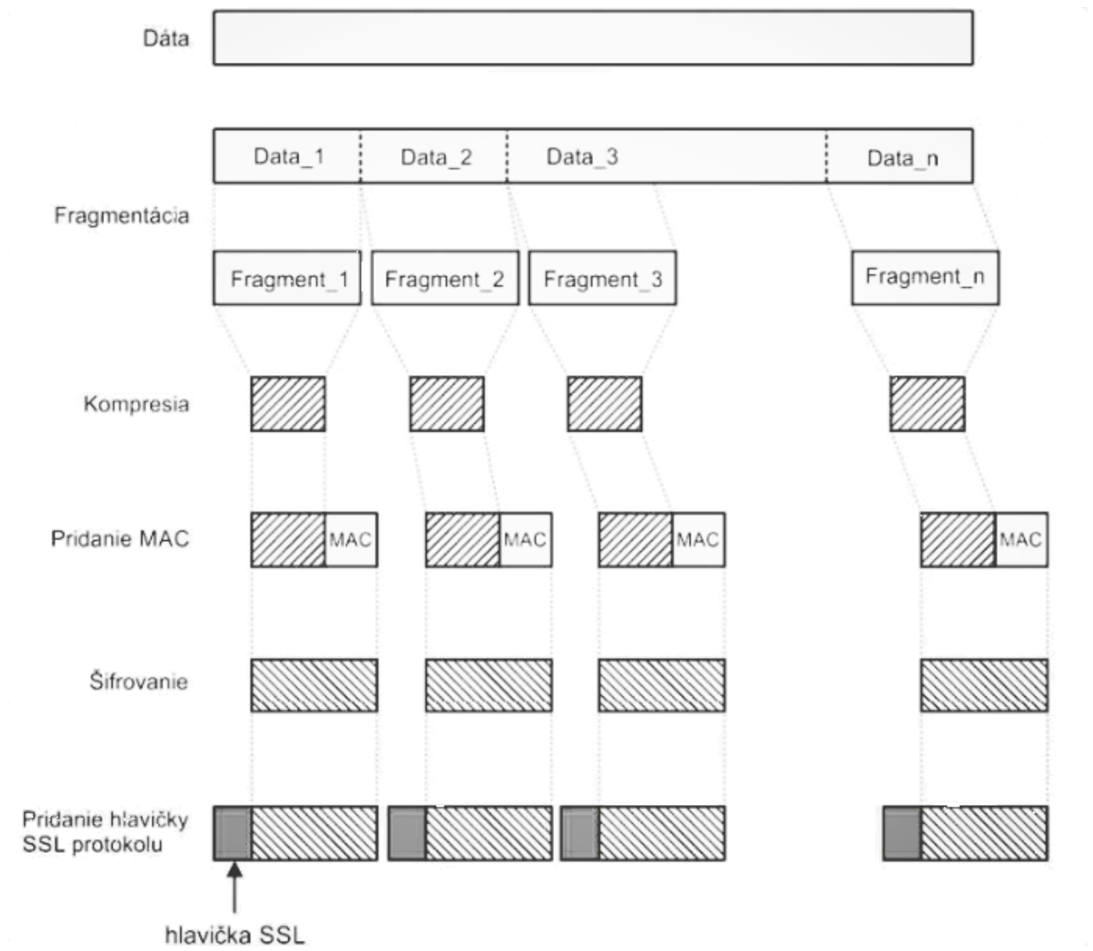
\includegraphics[width=0.7\linewidth]{figures/ssl}
	\caption{Prehľad operácií v SSL protokole}
	\label{ssl}
\end{figure}

Viac informácií o TLS protokole, jednotlivých verziách a optimalizáciách je možné nájsť na \cite{tls}. 

viac viac viac

\subsection{\acrfull{p2p}}
https://en.wikipedia.org/wiki/Point-to-Point\_Protocol

\subsection{\acrfull{mpls}}
\acrshort{mpls} by sme do slovenčiny mohli preložiť ako Multi-protokolové prepínanie štítkov. Samotný protokol pridáva k paketom tzv. MPLS hlavičku. Jej obsahom sú štítky\footnote{z ang. \textit{labels}}, na základe ktorých dochádza k smerovaniu a preposielaniu paketov. Týmto spôsobom nie je nutná ďalšia analýza paketov. Štítky neidentifikujú koncové body, ale virtuálne spojenia medzi viacerými uzlami. Označenie multi-protokolový má, pretože dokáže zapuzdrovať viacero sieťových protokolov. MPLS pracuje na pomedzi L2 a L3 vrstvy. Často sa zvykne označovať ako L2.5 protokol. Viac o tomto protokole je možné si prečítať na \cite{mpls}, \cite{mplstuke} a \cite{mplsrfc}.

\subsection{Charakteristika referenčných modelov}\label{crm}
V rámci  podkapitoly \ref{rm} je potrebné pred samotnou klasifikáciou vysvetliť pojmy Referenčný model prepojenia otvorených systémov\footnote{z ang. \textit{Open Systems Interconnection reference model}} (ďalej \acrshort{osi}) a Model opisujúci balíky internetových protokolov, známy ako, \acrshort{tcpip} referenčný model.

Úlohou uvedených referenčných modelov je vizualizácia postupu spracovania dát od používateľa až k ich odoslaniu zo zariadenia\footnote{z ang. \textit{end-to-end data communication}}. Pojem spracovanie dát znamená opísanie toho ako dochádza v jednotlivých abstraktných vrstvách k pretransformovaniu používateľských dát na súbor jednotiek a núl, ktoré sú následne odoslané do iného zariadenia. 

\acrshort{osi} Model vznikol v skorších fázach evolúcie počítačových sietí. Vychádza skôr z teoretického než praktického prístupu. Pozostáva zo 7 abstraktných vrstiev\footnote{z ang. \textit{layer}}:

\begin{enumerate}
	\item{\textbf{fyzická vrstva}} -- z ang. \textit{Physical Layer} (ďalej L1), 
	\item{\textbf{spojová vrstva}} -- z ang. \textit{Data Link Layer} (ďalej L2),
	\item{\textbf{sieťová vrstva}} -- z ang. \textit{Network Layer} (ďalej L3),
	\item{\textbf{transportná vrstva}} -- z ang. \textit{Transport Layer} (ďalej L4),
	\item{\textbf{relačná vrstva}} -- z ang. \textit{Session Layer} (ďalej L5),
	\item{\textbf{prezenčná vrstva}} -- z ang. \textit{Presentation Layer} (ďalej L6),
	\item{\textbf{aplikačná vrstva}} -- z ang. \textit{Application Layer} (ďalej L7).
\end{enumerate}

V schéme \ref{osi} sa nachádzajú stručne opísané jednotlivé činnosti vrstiev.
\begin{figure}[!h]
	\centering
	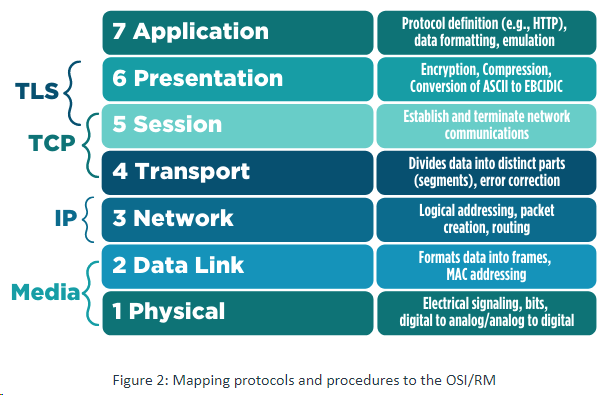
\includegraphics[width=0.8\textwidth]{figures/osi}
	\caption{https://www.comptia.org/blog/open-systems-interconnection-reference-model - dobry zdroj na rozsirenie}
	\label{osi}
\end{figure}


Čím je väčšie číslo vrstvy tým bližšie sa dáta nachádzajú pri používateľovi. Vďaka uvedeným vlastnostiam je tento model vhodnejší pri začiatku štúdia spracovania sieťových dát v počítači. Z rovnakého dôvodu sa taktiež viac stretávame s jeho použitím pri opise funkcionality riešenia ako s  \acrshort{tcpip} novším modelom.  Viac informácií o problematike nájde čitateľ v \cite{osi}.

Na druhej strane \acrshort{tcpip} model vznikol z praktického prístupu. Hlavný rozdiel je v počte abstraktných vrstiev, ktorý je v prípade \acrshort{tcpip} zmenšený na 4 vrstvy \cite{tcpip}. 
TCP/IP model je zobrazený pomocou schémy \ref{tcpipprot}. V uvedenej schéme sú znázornené aj niektoré z protokolov, ktoré sa na jednotlivých vrstvách používajú.

\begin{figure}[!ht]
	\centering
	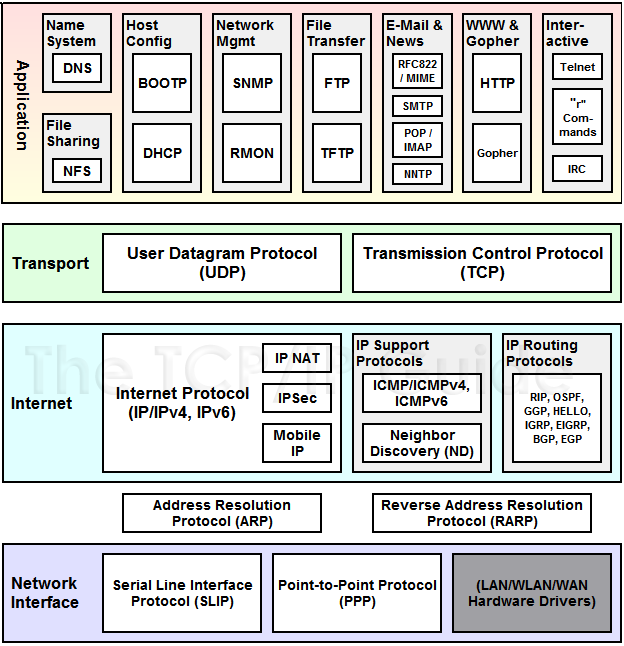
\includegraphics[width=0.9\textwidth]{figures/tcpipprot}
	\caption{Schéma TCP/IP modelu s niektorými protokolmi}
	\label{tcpipprot}
\end{figure}

\textbf{Aplikačná vrstva (L5-7)} zahŕňa protokoly používané väčšinou aplikácií na poskytovanie užívateľských služieb alebo výmenu aplikačných dát cez sieťové pripojenia, ktoré je vytvorené protokolmi na nižšej úrovni.  Spája vrstvy L5 až L7 OSI modelu. Príklady známych protokolov aplikačnej vrstvy sú \acrfull{http}, \acrfull{ftp}, \acrfull{smtp} a iné. Údaje, resp. dáta sú pri spracovaní kódované podľa L4 protokolov. Sú zapuzdrené do protokolových jednotiek transportnej vrstvy, tzv. \textbf{segmentov}.  

\textbf{Transportná vrstva (L4)} vytvára základné dátové kanály, ktoré aplikácie používajú na výmenu dát. Vrstva vytvára konektivitu medzi hostiteľmi, ktorá je nezávislá od siete, štruktúry užívateľských dát a smerovacích informácií. Konektivita na transportnej vrstve môže byť kategorizovaná ako orientovaná na spojenie, implementovaná v protokole \acrshort{tcp}, alebo \acrshort{udp} bez orientácie na spojenie. Uvedené protokoly sú stručne charakterizované nižšie, v tejto podkapitole. 

Protokoly v tejto vrstve zabezpečujú:
\begin{itemize}
	\item{riadenie chýb} -- z ang. \textit{error control} \cite{ec},
	\item{segmentáciu dát} -- z ang. \textit{segmentation} \cite{sd},
	\item{riadenie toku dát} -- z ang. \textit{flow control} \cite{fc},
	\item{riadenie preťaženia} -- z ang. \textit{congestion control} \cite{cc},
	\item{adresovanie aplikácií} -- z ang. \textit{application addressing} \cite{aa}.
\end{itemize}
Výstupom transportnej vrstvy sú segmenty, ktoré sú spracované v ďalšej vrstve referenčného modelu. 

\textbf{Internetová, resp. Sieťová vrstva (L3)} je zodpovedná za odosielanie paketov cez jednu alebo viac sietí. S touto funkcionalitou internetová vrstva umožňuje sieťovanie, prepojenie rôznych IP sietí a v podstate vytvára internet. Z L4 segmentov tvorí pakety, tak že pridá informácie potrebné na ďalšie smerovanie. 

\textbf{Linková vrstva (L2)} sa používa na presun paketov medzi rozhraniami internetovej vrstvy dvoch rôznych hostiteľov na rovnakom linku. Procesy vysielania a prijímania paketov na linke je možné konfigurovať. Zariadenia nazývané prepínače \footnote{z ang. \textit{switch}}, vykonávajú rámcovania\footnote{z ang. \textit{frame}}. Pripravujú pakety z L3 vrstvy na prenos pridaním ďalších informácií. Týmto úkonom vzniknú rámce. Tie sa prenášajú do fyzickej vrstvy a cez prenosové médium až k hostiteľovi. Fyzická vrstva predstavuje prvok, cez ktoré sú dáta prenášane. Napríklad optický a ethernetový kábel. 

Vyššie uvedené procesy prípravy dát sú znázornené pomocou schémy \ref{p1} a \ref{p2}.

\begin{figure}[!h]
	\centering
	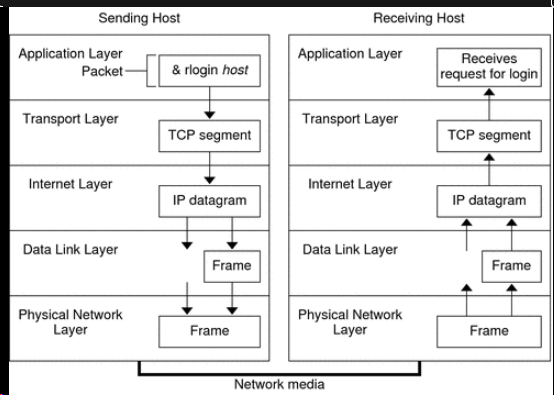
\includegraphics[width=0.7\linewidth]{figures/prenos1z2}
	\caption{spoj tento obrazok s nasledujucim do jedneho}
	\label{p1}
\end{figure}
\begin{figure}
	\centering
	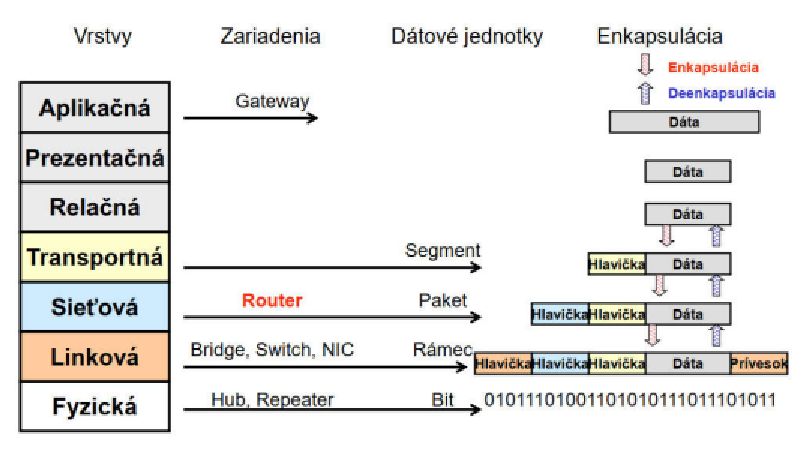
\includegraphics[width=0.7\linewidth]{figures/prenos2z2}
	\caption{spoj tento obrazok s predchadzajucim do jedneho, plus \ref{osi}}
	\label{p2}
\end{figure}
\newpage
\textbf{Protokol riadenia prenosu} (z ang. \textit{Transmission Control Protocol}, ďalej \acrshort{tcp}) je komunikačný protokol orientovaný na nadviazanie a udržanie sieťového spojenia medzi zariadeniami. Môže byť použitý pri úlohe príjímateľa aj odosielateľa (z ang. \textit{full-duplex}). Úlohou je spoľahlivý prenos dát medzi komunikantmi. Odoslanie a príjem dát je v rovnakom poradí. Protokol zároveň obsahuje mechanizmy na kontrolu výskytu chýb. Svoj názov má podľa dvoch najdôležitejších protokolov:
\begin{itemize}
	\item{Protokol riadenia prenosu} -- z ang. \textit{\acrlong{tcp}},
	\item{Internet protokol} -- z ang. \textit{\acrlong{ip}}. 
\end{itemize}

Na začiatku 21. storočia je 95\% paketov používaných na internete TCP. Bežné aplikácie používajúce TCP sú webové (HTTP/HTTPS protokoly), slúžiace na e-mailovú komunikáciu (SMTP/POP3/IMAP) a prenos súborov (z ang. \textit{File Transfer Protocol -- \acrshort{ftp}}). Minimálna dĺžka hlavičky TCP je 20 bajtov a maximálna dĺžka 60 bajtov. Po pridaní údajov TCP hlavičky k prenášaným dátam, vzniká tzv. \textit{segment}.

V súčasnosti je možne TCP protokol implementovať softvérovo aj hardvérovo. Pri prvom z uvedených je problémom závislosť na OS a následne aj vysoká vyťaženosť procesora pri príprave a spracovaní dát. Pri hardvérovom riešení je výhodou optimalizácia a implementácia bez potreby dodatočnej úpravy OS. Hardvérové implementácie sa realizujú pomocou koprocesorov umiestnených vo vnútri procesora. Následkom toho môžeme dnes bežne pozorovať umiestnenie spomenutých zariadení na našich zariadeniach.

Podrobnejšie informácie o TCP protokole je možné nájsť na \cite{tcp2}. V uvedenej publikácií sa nachádza opis TCP hlavičky, metódy nadviazania a ukončenia spojenia. Obdobne je spomenuté ako dochádza k prenosu dát pomocou sekvenčných čísel. Ak má používateľ nejasnosti v fungovaní TCP protokolu, odporúča sa danú publikáciu prečítať.

\textbf{Používateľský datagramový protokol} (z ang. \textit{User Datagram Protocol}, ďalej \acrshort{udp}) je jedným zo základných komunikačných \acrshort{ip} protokolov. Používa sa na odosielanie správ iným hostiteľom v sieti. Správy sú prenášané ako datagramy v paketoch. \acrshort{udp} nevyžaduje predchádzajúcu komunikáciu na nastavenie komunikačných kanálov alebo dátových ciest. Používa jednoduchý komunikačný model bez spojenia s minimom protokolových mechanizmov. Poskytuje kontrolné súčty pre integritu údajov a čísla portov na adresovanie rôznych funkcií v zdroji a cieli datagramu. 

Narozdiel od \acrshort{tcp}) neposkytuje žiadnu záruka doručenia správy alebo duplicitnej ochrany. 
\acrshort{udp}) je vhodný na účely, kde kontrola a oprava chýb buď nie sú potrebné, alebo sa vykonávajú v aplikácii. Aplikácie citlivé na čas často používajú UDP, pretože zahadzovanie paketov je vhodnejšie ako čakanie na pakety oneskorené v dôsledku opätovného prenosu. Príklad použitia môžu byť streamovacie služby. 
Podrobnejšie informácie o \acrshort{udp}) protokole nájde čitateľ v \cite{udp}.

\section{Klasifikácia VPN sietí}
V súčasnosti má čitateľ k dispozícií veľa rôznych internetových zdrojov o problematike VPN. Uvedené sú rôzne možnosti klasifikácie VPN siete. V rámci tejto práce klasifikujeme VPN siete podľa logickej topológie, použitých protokolov a vrstiev, na ktorých sú postupy aplikované. Obsahom tejto podkapitoly je rozdelenie a opis jednotlivých typov VPN sieti. V závere kapitoly čitateľ nájde sumárne rozdelenie VPN sieti v tejto práci, znázornené pomocou schémy.  
\subsection{Rozdelenie VPN sieti podľa logickej topológie}
 Podľa topológie, v ktorej VPN spojenie prebieha rozdeľujeme VPN do 3 kategórií: 
\begin{itemize}
	\item \textbf{VPN rovný s rovným} -- \textit{z ang. Peer to Peer VPN},
	\item \textbf{VPN klient a server} -- \textit{z ang. Client to Server VPN}, 
	\item \textbf{VPN sieť so sieťou} -- \textit{z ang. Site to Site VPN}.
\end{itemize}

\subsubsection{VPN rovný s rovným}
Uvedený spôsob vytvára zabezpečený tunel medzi dvoma rovnocennými uzlami, resp. zariadeniami\footnote{z ang. \textit{peers}}, ktorý spoločne komunikujú cez verejnú sieť. Medzi zariadeniami je vytvorený tunel. Každý koniec má priradenú svoju IP adresu. Z uvedeného modelu vyplýva aj následná limitácia. VPN tunel vznikne iba medzi dvoma komunikujúcimi zariadeniami. Z toho dôvodu nie je toto použitie časté. Na obrázku \ref{p2p} je znázornený uvedený typ VPN spojenia. 
\begin{figure}[!ht]
	\centering
	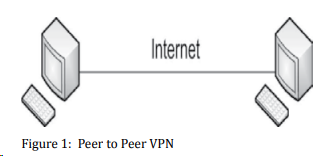
\includegraphics[width=.7\textwidth]{figures/p2p}
	\caption{}
	\label{p2p}
\end{figure}
 
\subsubsection{VPN Klient a Server}
Tento typ spojenia pozostáva z pripojenia medzi nerovnocennými dvoma alebo viacerými zariadeniami. Najjednoduchší model musí pozostávať z jedného VPN servera a VPN klienta. Princíp spočíva vo vytvorení zabezpečeného tunela, ktorý je použitý na prenos dát medzi uvedenými zariadeniami. Zároveň je však možné vytvoriť $1:N$ takýchto spojení. $N$ reprezentuje počet VPN klientov, resp. prepojení, ktorý VPN Server dokáže nadviazať. Tento parameter je závislý najmä od hardvérových prostriedkov daného servera.

Úloha Klienta spočíva v presmerovaní všetkej svojej sieťovej komunikácie cez zabezpečený tunel, ktorý vznikol medzi ním a Serverom. Tento úkon je najčastejšie realizovaný presmerovaním trafiky cez sieťovú bránu\footnote{z ang. \textit{GateWay}} (ďalej \acrshort{gw}). V danom \acrshort{os}, na ktorom VPN klient beží, je teda potrebné zmeniť IP adresu \acrshort{gw} na adresu VPN servera. Vďaka tomu nastane presmerovania komunikácie. Tento úkon je väčšinou realizovaný programovo pomocou aplikácií. Typicky nastolia spojenie medzi Klientom a Serverom. Následne upravia sieťové nastavenia systému. Spomenuté úkony sú vysoko závislé od \acrshort{os} a daného programovacieho jazyka, prostredníctvom ktorého sú úpravy realizované. 
Úloha Servera na druhej strane spočíva vo vytvorení možnosti pripojenia pre jedného alebo viacerých klientov. Následne Server zastupuje klientovu prítomnosť v danej sieti. Teda spracúva požiadavky Klienta a komunikuje s ostatnými zariadeniami. Komunikácia ďalej však už nie je zabezpečená pomocou šifrovania alebo tunelu. Tento fakt je znázornený na obrázku \ref{c2s}.   

\begin{figure}[!ht]
	\centering
	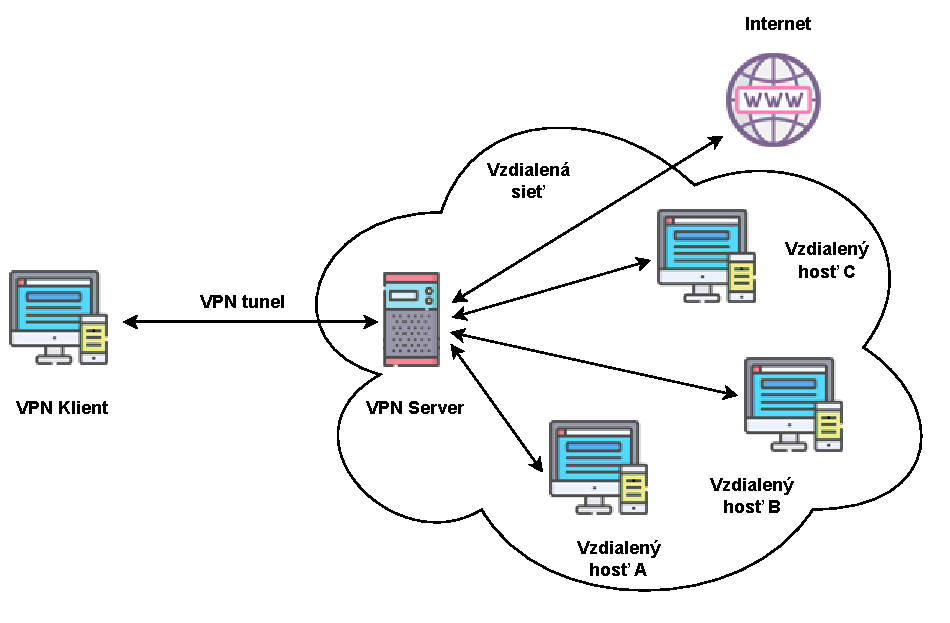
\includegraphics[width=.7\textwidth]{figures/c2s}
	\caption{potrebne prerobenie nech sa to nepodoba na 1.1 alebo vyhodit/upravit 1.1}
	\label{c2s}
\end{figure}
V súčasnosti je tento spôsob považovaný za najviac používaný v oblasti korporátneho sveta. VPN server slúži ako vstupná brána do internej siete. Vďaka tomu je možné sprístupniť zdroje pre používateľov z rôznych oblastí sveta. Používateľ sa taktiež môže stretnúť s pomenovaním model \textbf{uzol k sieti}, resp. z ang \textit{point-to-site}. Obidva pojmy sú správne a predstavujú rovnakú myšlienku zapojenia VPN.  
\subsubsection{Sieť so Sieťou VPN}
VPN model Sieť so Sieťou vytvára zabezpečený tunel medzi dvoma rôznymi sieťami naprieč verejnou sieťou. Model pozostáva z 2 zariadení -- VPN servera a VPN Koncentrátora\footnote{z ang. \textit{VPN Concentrator}}.

VPN Koncentrátor je typ sieťového zariadenia, ktoré poskytuje zabezpečené VPN spojenie a doručenie dát. Zvyčajne je to špecializovaný smerovač\footnote{z ang. \textit{router}}. Dokáže vytvárať veľké množstvo VPN tunelov. Používa sa na nastolenie VPN modelu sieť so sieťou. Funkcionalita koncentrátora pozostáva z: 
\begin{itemize}
	\item{nastolenie a konfiguráciu VPN tunela} -- z ang. \textit{Establish and Configure tunnels},
	\item{autentizáciu používateľa}-- z ang. \textit{Authenticate users},
	\item{priradenie IP adries používateľov k tunelom} -- z ang. \textit{Assign tunnel/IP addresses to users},
	\item{šifrovanie a dešifrovanie dát} -- z ang. \textit{Encrypt and Decrypt data},
	\item{zabezpečiť integritu doručenia} -- z ang. \textit{Ensure end-to-end delivery of data}.
\end{itemize}

Model Sieť so sieťou je používaný najmä pri spojení vedľajšej pobočky s hlavnou, ktoré sa nachádzajú na rozdielnych geografických lokalitách. Pomocou schémy \ref{sts} je znázornený tento model. 

 \begin{figure}[!ht]
 	\centering
 	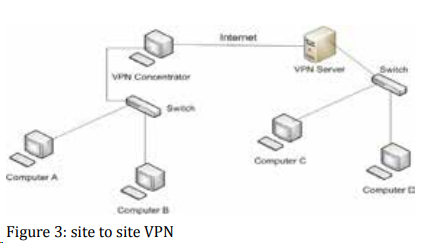
\includegraphics[width=.7\textwidth]{figures/sts}
 	\caption{rearanzovat}
 	\label{sts}
 \end{figure}  

Informácia z tejto podkapitoly boli čerpané z \cite{vpntech}.  
\subsection{Rozdelenie VPN sieti podľa vrstiev referenčného modelu}\label{rm}
VPN siete môžeme klasifikovať podľa vrstvy (ďalej \acrshort{l}) referenčného modelu, na ktorej dochádza k šifrovaniu dát. Stručná charakteristika referenčných modelov je obsahom podkapitoly \ref{crm}.

Klasifikácia VPN sietí podľa \acrshort{osi} modelu:
\begin{itemize}
	\item{\textbf{L2 VPN}} -- VPN na spojovej vrstve,
	\item{\textbf{L3 VPN}} -- VPN na sieťovej vrstve,
	\item{\textbf{L4 VPN}} -- VPN na transportnej vrstve.
\end{itemize}

Pri implementácií VPN komunikácie medzi zariadeniami je pre pochopenie dôležité určiť aké dáta vstupujú do šifrovacieho algoritmu. Pomocou tejto informácie a klasifikácie vyššie následne dokážeme zaradiť do určitej kategórie. Na schéme \ref{osidata} je možné si všimnúť aké dáta sú výstupom jednotlivých vrstiev. (spoj dva obrazky do jedneho netreba zbytocne dva)

\begin{figure}[!h]
	\centering
	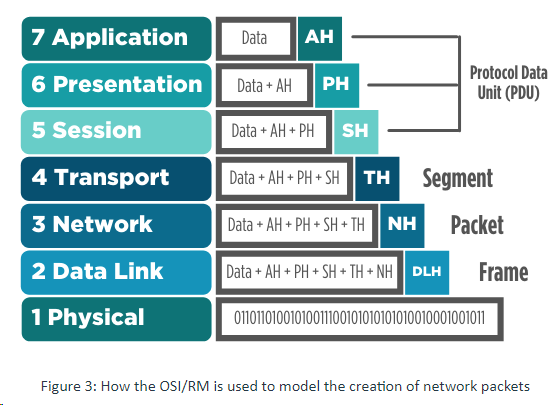
\includegraphics[width=0.7\textwidth]{figures/osidata}
	\caption{zakomponovat k osi vysvetleniu}
	\label{osidata}
\end{figure}

Princíp použitia bloku na šifrovanie je znázornený pomocou schémy \ref{sifr}.

\begin{figure}[!h]
	\centering
	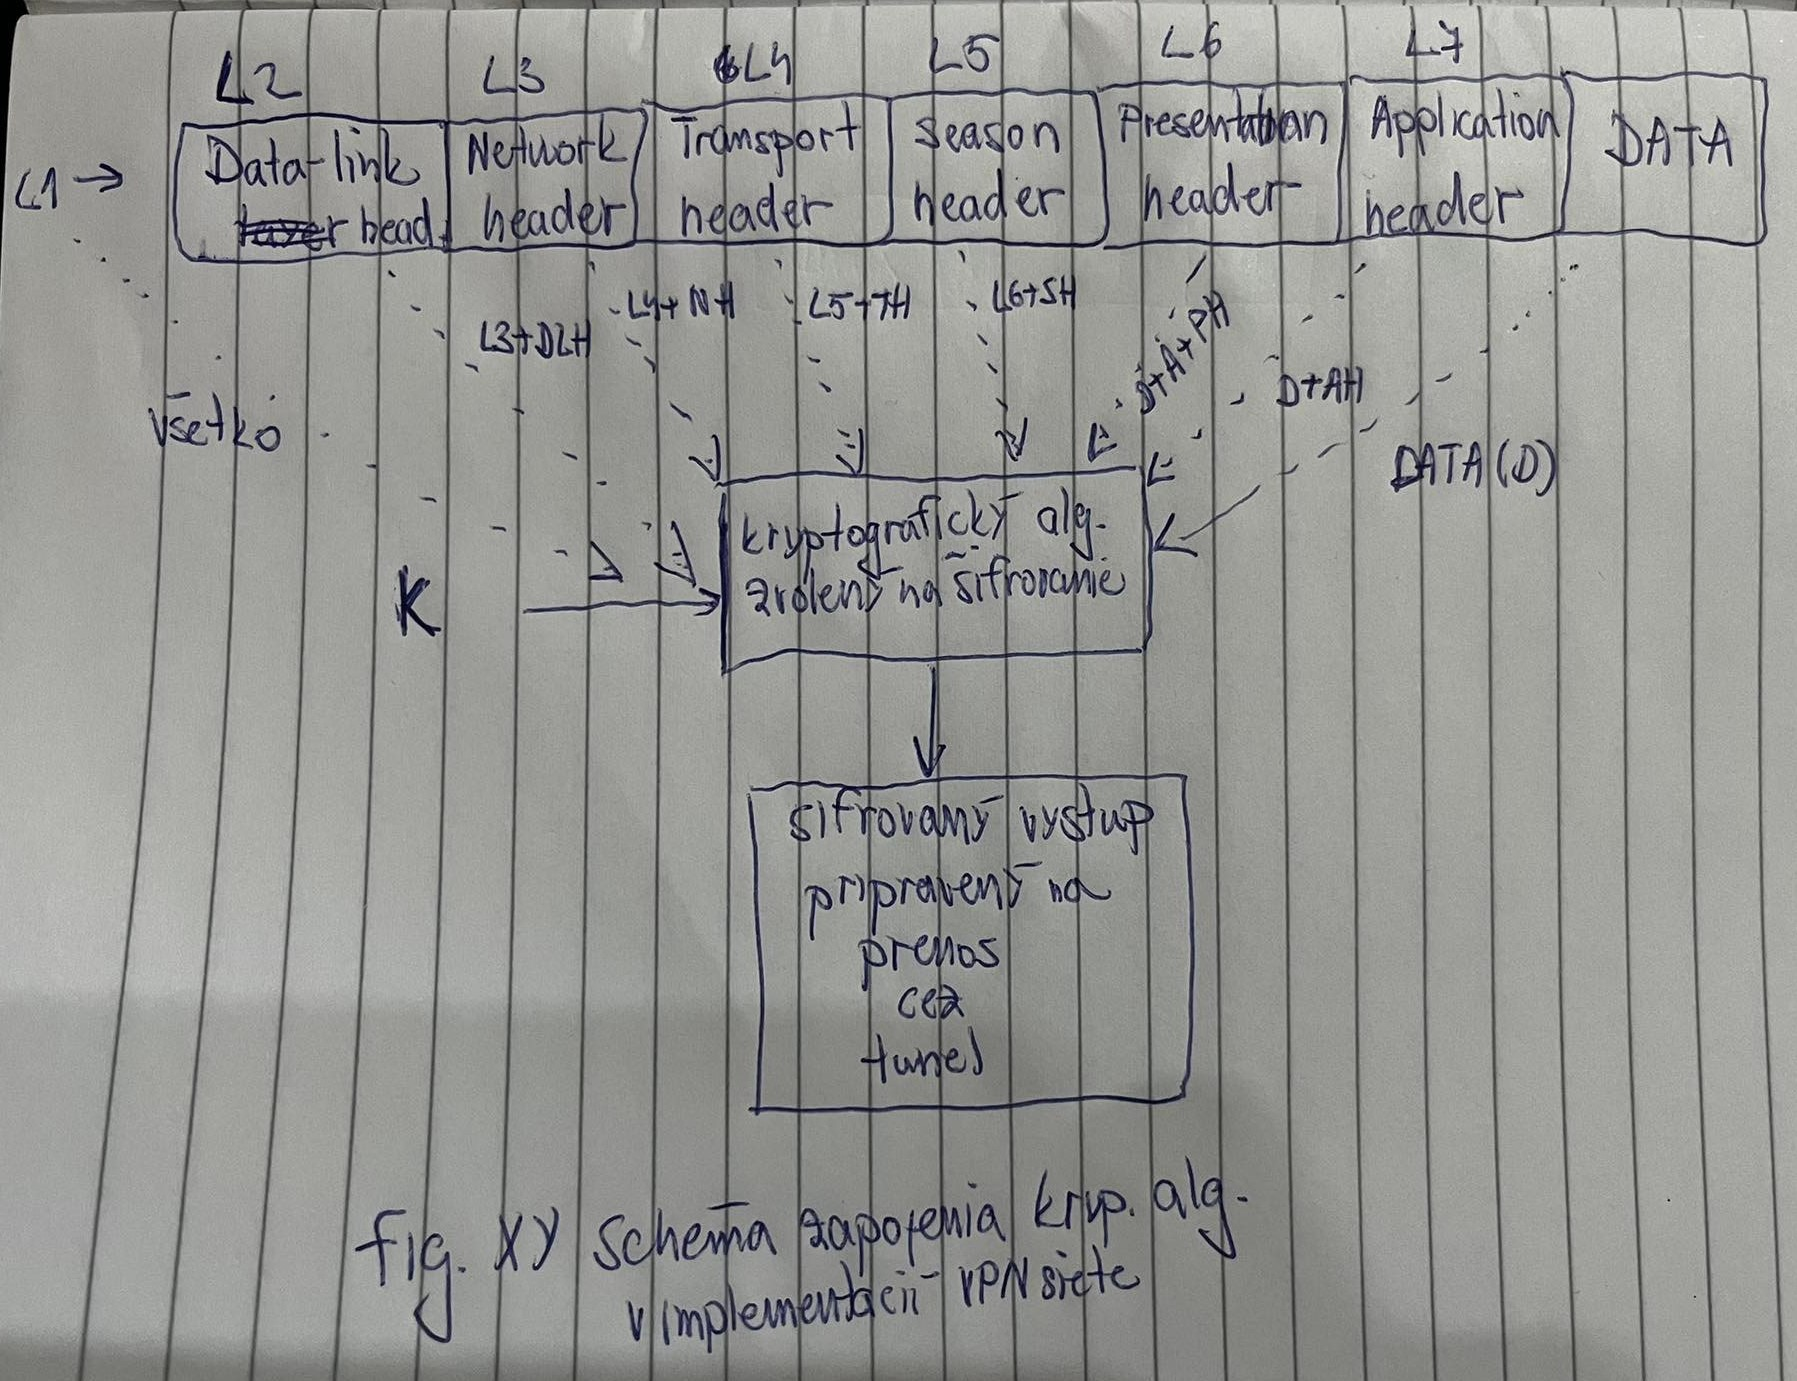
\includegraphics[width=0.7\textwidth]{figures/sifr.jpg}
	\caption{potreba upravy iba na spoemnute vrstvy}
	\label{sifr}
\end{figure}

Zo schémy je viditeľné, že spracovaním nižšej vrstvy dochádza k zväčšeniu bloku dát, ktoré je potrebné šifrovať. To môže negatívne ovplyvniť výslednú rýchlosť celého systému. Okrem uvedenej vlastnosti je dalším problémom prenos vrámci rôznych sieti. Každé zariadenie, ktoré smeruje dáta by muselo repetitívne šifrovať a dešifrovať čím by v danej implementácií vzniklo viac rizikových miest pre potencionálny útok. Z uvedených dôvodov je preto najrozšírenejší spôsob zapojenia šifrovacieho bloku na pomedzi L3 až L4 vrstvy. Smerovanie ostáva bez zásahu a k dešifrovaniu dochádza až na konečnom zariadení, prípadne v aplikácií na samotných dátach.

Typický sa s L2 a L3 VPN sieťami môže používateľ stretnúť na špecializovaných sieťových zariadeniach. Konkrétne na routroch a switchoch. Prvé z uvedených je využívané najmä pri smerovaní, respektíve určení cesty smerom von z lokálnej siete až k cieľovej destinácií. Tento úkon je vykonaný za pomoci aplikácie smerovacích protokolov. Router je možné použiť aj na smerovanie v rámci lokálnej siete. V porovnaní so switchom však nedosahuje porovnateľný výkon. Na druhej strane klaasický switch je možné použiť len vrámci lokálnej siete. V súčasnosti sa používajú aj tzv. L3 switche. V porovnaní s routrom je ich prednosťou vyššia rýchlosť spracovania prichádzajúcich paketov pri väčšom počte pripojených zariadení.        

\section{Protokoly vo VPN sieťach} 
V predchádzajúcej podkapitole sme klasifikovali VPN siete na základe zapojenia kryptografického bloku do OSI referenčného modelu. V tejto podkapitole pomocou uvedeného rozdelenia, zaradíme a charakterizujeme zopár protokolov, ktoré sa typicky používajú vo VPN sieťach. Pred začiatkom by som rád čitateľa upozornil, že aktuálne neexistuje svetový štandard na vytváranie VPN spojení. Dôsledkom toho existuje veľké množstvo rôznych protokolov. Vrámci tejto podkapaitoly si predstavíme niektoré z nich. 

\subsection{\acrfull{pptp}}

?nerozumiem?PPTP enables on-demand, virtual private networks over the Internet or other public TCP/IP-based data networks ??\\

\acrshort{tcpip} sieťový protokol \acrshort{pptp} poskytuje zabezpečuje bezpečný prenos dát z klienta do privátneho servera vo VPN sieti. Jedná sa o starší Microsoft L2 protokol, ktorý bol definovaný v roku 1996. Je rozšírením L2 \acrshort{p2p} protokolu. \acrshort{pptp} zapuzdruje \acrshort{p2p} pakety do  IP datagramov. Následne ich prenáša cez sieť. Typicky pozostáva spojenie z 3 zariadení, ktoré sú znázornené na schéme \ref{ptptun} a \ref{pptpcon}. 

% TODO: \usepackage{graphicx} required
\begin{figure}[h]
	\centering
	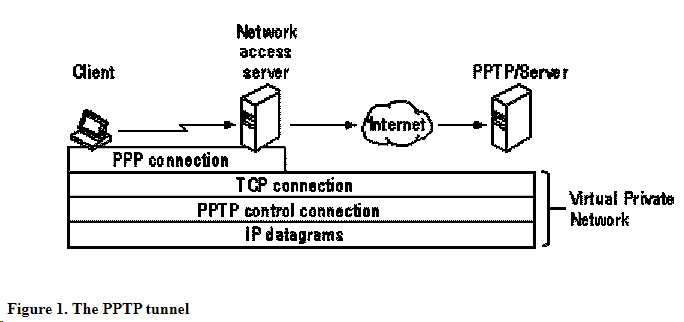
\includegraphics[width=0.7\textwidth]{figures/ptptun}
	\caption{Architektura PPTP siete - PPTP je az od nas do PS}
	\label{ptptun}
\end{figure}
% TODO: \usepackage{graphicx} required
\begin{figure}[h]
	\centering
	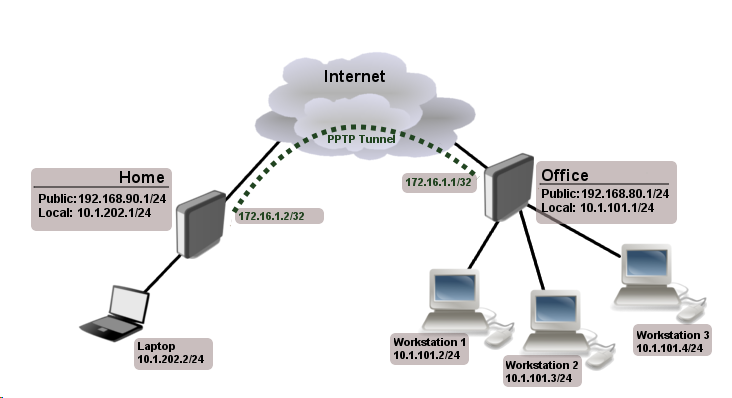
\includegraphics[width=0.7\textwidth]{figures/pptpcon}
	\caption{lepsi obrazok}
	\label{pptpcon}
\end{figure}

Zabezpečenie prenosu pomocou \acrshort{pptp} pozostáva typicky z 3 po sebe nasledujúcich procesov:
\begin{enumerate}
	\item{PPP pripojenie a komunikácia } -- z ang. \textit{PPP Connection and Communication},
	\item{riadenie spojenia pomocou PPTP protokolu} -- z ang. \textit{PPTP Control Connection},
	\item{prenos dát PPTP tunelom} -- z ang. \textit{PPTP Data Tunneling}.
\end{enumerate}
Prechod medzi procesmi je možný len ak došlo k úspešnému dokončeniu predchádzajúceho kroku. V prvom procese sa PPTP klient pripája k serveru s prístupom na internet\footnote{z ang. \textit{Network Access Server}} (ďalej \acrshort{nas}). Používa sa pri tom PPP protokol, ktorý nastolí spojenie a zašifruje pakety. V druhom kroku následne vznikne TCP pripojenie medzi NAT a PPTP serverom. Použitý je port 1723. Uvedeným postupom nám vznikne medzi zariadeniami PPTP Tunel. Po úspešnom vytvorení konektivity dochádza k zapuzdrovaniu prichádzajúcich zašifrovaných PPP dát do PPTP protokolu a ich prenosu cez tunel. PPTP zapuzdruje dáta do tzv. IP datagramov, ktoré už obsahujú zašifrovaný PPP paket. Datagramy su vytvorené pomocou \acrshort{gre} protokolu, ktorý bol opísaný v \ref{gre}. Na schéme \ref{pptpdat} je znázornená schém PPTP Paketu. 

\begin{figure}
	\centering
	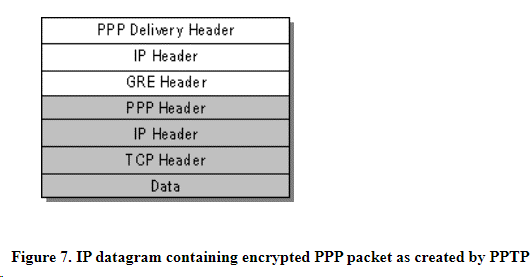
\includegraphics[width=0.7\textwidth]{figures/pptpdat}
	\caption{sede sifrovane biele nie }
	\label{pptpdat}
\end{figure}

PPTP Server po prijatí dáta rozbalí, dešifruje PPP paket a následne ho smeruje v rámci lokálnej siete.

Je dôležité poznamenať, že PPTP klient môže mať priamy prístup na internet. V uvedenom prípade sa nevytvára prvotné PPP spojenie až k internetovému poskytovateľovi.
Viac informácií o protokole PPTP nájde čitateľ na \cite{rfc2637} a \cite{pptp}, ktoré boli zdrojom pri tvorbe tejto podkapitoly.
\subsubsection{Bezpečnosť a použitie protokolu} 
Protokol vznikol v júny 1996. Implementácia poskytuje používateľovi:
\begin{itemize}
	\item{\textbf{Autentizáciu}} -- z ang. \textit{Authentication}, overenie totožnosti používateľa pomocou mena a hesla. Na výber boli autentizačné protokoly \textit{Challenge Handshake Authentication Protocol} (\acrshort{chap}) \cite{chap}, \textit{MicroSoft Challenge Handshake Authentication Protocol} (\acrshort{mschap}) \cite{mschap} a \textit{Password Authentication Protocol} (\acrshort{pap}) \cite{pap}.  
	\item{\textbf{Kontrolu prístupu}} -- z ang. \textit{Access Control}, po úspešnej autentizácií je následne prístup používateľa riadený na základe pravidiel a politiky prístupu daného OS. 
	\item{\textbf{Šifrovanie dát}} -- z ang. \textit{Data Encryption}, je vykonané pomocou vopred zdieľaného kľúča, ktorý sa získa odvodením z hašovanej hodnoty uloženého hesla používateľa. Haš je vstupom do prúdovej šifry RC4 \cite{rc4} a výstupom je  40-bitový kľúč relácie. 
	\item{\textbf{Filtrovanie PPTP paketov}} -- z ang. \textit{PPTP Packet Filtering}, možnosť zapnutia filtrovania paketov len autentizovaných PPTP klientov.
	\item{\textbf{Preddefinované Firewall pravidla pre PPTP}} -- z ang. \textit{PPTP with Firewalls and Routers}, PPTP má štandardne definovaný TCP port 1723 a ID 47 v IP protokole. Vďaka tomu je možné jednoducho presmerovať tok dát.
\end{itemize} 

Protokol je aktuálne štandardne zahrnutý v každej distribúcií \acrshort{os} Windows aj Linux. Pri vytváraní VPN siete teda používateľ môže zvoliť uvedený protokol na zabezpečený prenos dát v lokálnej, ale aj naprieč verejnou sieťou. Výhodou protokolu je vysoká kompatibilita naprieč rôznymi platformami. Nevýhodou je veľké množstvo zraniteľných miest, možností zneužitia a použitie starších kryptografických algoritmov. Aktuálne existujú protokoly poskytujúce lepšiu bezpečnosť ako uvedená implementácia. Z uvedených dôvodov sa tento protokol neodporúča používať.


\subsection{\acrfull{l2tp}}
Ďalším z VPN tunelovacích protokolov je \acrshort{l2tp}. Špecifikovaný bol v roku 2000 v dokumente \acrshort{rfc}\footnote{z ang. \textit{Request For Comments}} 2661 \cite{rfc2661}. Inšpirovaný dvoma staršími protokolmi \acrshort{l2f}\footnote{z ang. \textit{Cisco Layer 2 Forwarding Protocol}} \cite{rfc2341} a PPTP.   

L2TP sieť pozostáva primárne z 3 zariadení:
\begin{enumerate}
	\item{\textbf{PPP terminál}} -- ľubovoľné zariadenie na vykonanie PPP enkapsulácie na dáta a pripojenie k \acrshort{lac}\footnote{z ang. \textit{L2TP access concentrator}}. Môže to byť aj samotné zariadenie, ktoré sa pripája. 
	\item{\textbf{L2TP prístupového servera}} -- \acrshort{lns}\footnote{z ang. \textit{L2TP Network Server}}, jeden z koncov tunela, ktorý deenkapsuluje dáta a poskytuje prístup do lokálnej sieti. Na zariadení prebieha autentizácia používateľa, nastolenie PPP relácie\footnote{z ang. \textit{session}} a L2TP tunela s \acrshort{lac}. Nasadzuje sa na hranici medzi privátnou a verejnou sieťou, zvyčajne ako sieťová brána na opustenie danej súkromnej siete\footnote{z ang. \textit{gateway}}. Obdobne poskytuje funkcionalitu prekladu adries z privátnych do verejných a opačne. Uvedená funkcionalitá sa nazýva \acrfull{nat}. Viac o tomto protokole je dostupné na \cite{nat}.   
	\item{\textbf{L2TP koncentrátora}} -- \acrshort{lac}, zariadenie umiestnené medzi LNS a clientom. Služí na preposielanie paketov oboma smermi. V smere k LNS vytvára L2TP tunel. LAC server môže byť nasadený aj na PPP termináli a pracovať ako \acrshort{poe}\footnote{z ang. \textit{PPP Over Ethernet}} server. Zvyčajne je koncentrátor nasadený na \acrshort{nas}, ale je možné ho nasadiť na ľubovoľné sieťové zariadenie.
\end{enumerate}
V schéme \ref{l2tp} je znázornené ako sú spomenuté zariadenia zapojené v logickej topológií. Na schéme je znázornený aj proces enkapsulácie PPP paketov, prenosu dát naprieč tunelom a následnej deenkapsulácie. 
% TODO: \usepackage{graphicx} required
\begin{figure}
	\centering
	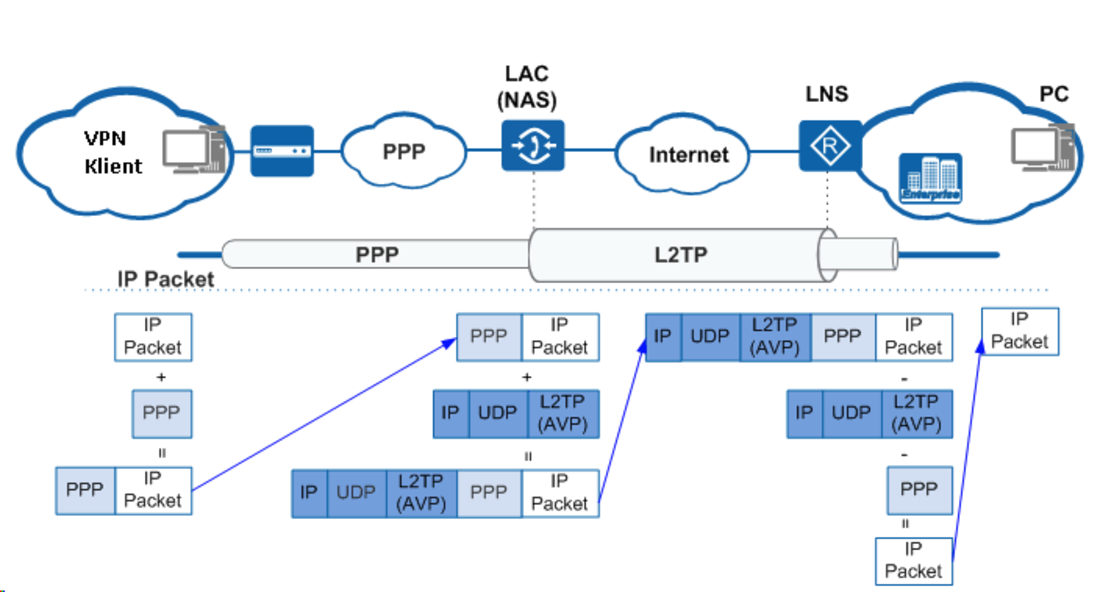
\includegraphics[width=0.7\textwidth]{figures/l2tp}
	\caption{}
	\label{l2tp}
\end{figure}

L2TP používa namiesto TCP protokolu UDP, ktorého výhodou je rýchlejší prenos bez kontroly prijatia na druhej strane spojenia.  
Pri vzniku tunela používa UDP port 1701. Iniciátor tohto procesu následne vyberá náhodne z nečinných portov a smeruje nim pakety s portom 1701. Prijímač po prijatí paketu taktiež náhodne určí nečinný port a preposiela ním pakety prijaté iniciátorom. Takto zvolené portové čísla sa používajú až kým nie je komunikácia cez tunel ukončená. 

L2TP vytvára 2 druhy spojenia počas vytvárania konektivity medzi LAC a LNS. 
\begin{itemize}
	\item{\textbf{tunelové spojenie}} -- z ang. \textit{tunnel connection}, napomáha k nastoleniu viacero tunelov medzi zariadeniami. Pozostáva z jedného alebo viacerých relačných spojení. Žiadosť o vytvorenie vytvára LAC server po prijatí PPP žiadosť od vzdialeného používateľa. LAC a LNS si vymenia informácie potrebné na vznik spojenia ako sú napríklad autentizačné informácie tunela a ID. Po úspešnom vyjednávaní\footnote{z ang. \textit{negotiation}} vznikne tunel, ktorý je identifikovateľný pomocou dohodnutého ID.  
	\item{\textbf{relačné spojenie}} -- z ang. \textit{session connection}, reprezentuje PPP spojenie naprieč tunelom. Môže vzniknúť až keď je tunel úspešne vytvorený.	
\end{itemize}     
Po vytvorení oboch spojení následne odchádza k prenosu zapuzdrených PPP paketov naprieč týmto tunelom.

L2TP ponúka kompatibilitu pre mnohé platformy a jednoduchú konfiguráciu. OS Windows, Linux a Mac majú tento protokol zabudovaný v sebe. Výhodou je použitie UDP, vďaka tomu je možné protokol používať aj v nestabilnom sieťovom prostredí.
Nevýhodou je zníženie prenosovej rýchlosti. L2TP používa taktiež vopred zdieľané kľúče a v prípade ak sa nezhodujú, tak dochádza k zastaveniu chodu. L2TP je podporuje iba limitovaný počtet portových čísel. Samotná implementácia L2TP neposkytuje, respektíve nezabezpečuje žiadne šifrovanie alebo autentizáciu paketa. Na zabezpečenie sa používa v kombinácií s iným protokolom. Veľmi známa je implementácia L2TP/IPSec. 

V roku 2005 vznikla 3. verzia protokolu, ktorá priniesla zväčšenie dĺžky ID v L2TP hlavičke, zo 16 na 32 bitov. Rozšírenie tunelového autentizačného mechanizmu a oddelenie L2TP dát súvisiacich s PPP protokolom. Viac o tomto upravenom protokole je možné nájsť na \cite{l2tpv3}.
  
Viac informácií o L2TP problematike je možné nájsť v \cite{l2tp}, \cite{rfc2661}, \cite{l2tphuawei}, odkiaľ boli informácie z tejto podkapitole čerpané. 

\subsection{Internet Protocol Security (\acrshort{ipsec})}
\acrshort{ipsec} je otvorený štandard. Vďaka tomu vďačí za veľkú popularitu a pravidelné aktualizácie kryptografických algoritmov. Protokol sa využíva na zabezpečenie bezpečnosti v sieti. IPSec môžeme klasifikujeme ako L3 protokol nakoľko pracuje s dátami zo sieťovej vrstvy. Má dva režimy:
\begin{itemize}
	\item{\textbf{transportný režim}} -- po prijatí paketu z vyššej vrstvy sú smerovacie dáta zachované a na základe nich sú dáta odosielané ďalej. K zvyšným dátam je pridaná hlavička použitého IPSec protokolu. Princíp pridania dát k paketu je znázornený na \ref{iptransport}  
	\item{\textbf{tunelovací režim}} -- zapuzdruje paket z vyššej vrstvy. Pridáva novú IP hlavičku a hlavičku IPSec protokolu k pôvodnému nezapuzdrenému paketu. Uvedená skutočnosť je zobrazená na obrázku \ref{iptunel}
\end{itemize}
% TODO: \usepackage{graphicx} required
\begin{figure} [!h]
	\centering
	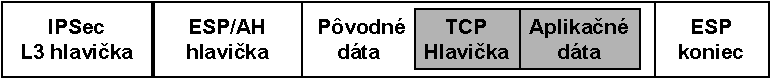
\includegraphics[width=0.7\textwidth]{figures/iptransport}
	\caption{IPSec transportný režim}
	\label{iptransport}
\end{figure}
% TODO: \usepackage{graphicx} required
\begin{figure} [!h]
	\centering
	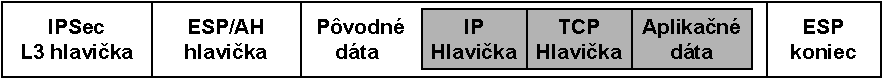
\includegraphics[width=0.7\textwidth]{figures/iptunel}
	\caption{IPSec tunelovací režim}
	\label{iptunel}
\end{figure}


Za účelom poskytnutie zabezpečeného spojenia, protokol vykonáva autentizáciu, šifrovanie a vyjednávanie, resp. výmenu potrebných kľúčov. Jednotlivé činnosti sú realizované pomocou týchto IPSec protokolov:
\begin{itemize}
	\item{\textbf{Autentizačná hlavička}} -- z ang. \textit{Authentication Header}, pridáva k prepravovanému paketu dáta na zabezpečenie dátovej integrity a pôvodu. Chráni proti z ang. \textit{Replay attack} \cite{repa}. Dáta v tomto režime nie sú šifrované. AH hlavička je vygenerovaná v závislosti od toho v akom IPSec režime je protokol použítý.    
	\item{\textbf{Bezpečnostné zapuzdrenie nákladu}} -- z ang. \textit{Encapsulating Security Payloads}, narozdiel od AH, ESP aj šifruje dáta z vyššej vrstvy. Vďaka tomu dochádza k zabezpečeniu dôvernosti, datovej integrity a autentizácie pôvodu. Výsledná hlavička závisí od dát zo sieťovej vrstvy a konfigurácie IPSec.    
	\item{\textbf{\acrlong{isakmp}}} -- ďalej \acrshort{isakmp}, protokol na autentizáciu a výmenu kľúčov. Slúži taktiež na vytvorenie parametra \acrshort{sa}, ktorý sa používa v hlavičke \acrshort{ah}/\acrshort{esp}.
\end{itemize}

IPSec je možné nakonfigurovať, tak aby používal \acrshort{ah} a \acrshort{esp} selektívne alebo aj súčasne. V závislosti od konfigurácie následne dochádza k zapuzdrovaniu prichádzajúceho paketu. Používateľ má na výber viacero štandardných kryptografických algoritmov. Príkladmi sú \acrshort{aes} \cite{aes}, \acrshort{rsa} \cite{rsa}, Diffie-Hellman \cite{dh} a  eliptické krivky (\acrshort{ecdsa} \cite{ecdsa} aj \acrshort{ecdh} \cite{ecdh}).

Nabudúce sa opytat ci biks predmet moze byt zdroj alebo ine. \cite{biks}

\subsection{Secure Socket Tunneling Protocol (\acrshort{sstp})}
SSTP je bežný L2 VPN protokol, ktorý zapuzdruje PPP ramce cez \acrshort{https} protokol \cite{https}. Spolieha sa na \acrshort{ssl}, resp. \acrshort{tls}, ktoré sú opísané v úvode práce. Vďaka tomu umožňuje ľahší prechod cez väčšinu firewallov a proxy brán. Teda blokovanie takto vytvoreného VPN spojenia je pre poskytovateľov internetu a správcov siete zložitejšie. 

SSTP bol vytvorený v roku 2007 spoločnosťou Microsoft. Primárne pre platformu Windows. Cieľom bolo poskytnúť bezpečnejšiu náhradu za PPTP a L2TP. V súčasnosti sa považuje za jeden zo štandartných protokolov. Je dostupný vo viacerých operačných systémoch vrátane Linuxu a BSD. Pravidelne udržiavaný o čom svedčia aj priebežná aktualizácia dokumentácie na Microsoft dokumentačných stránkach. Informácie k tejto podkapitole boli čerpané z \cite{mssstp}. V uvedenom zdroji je možné nájsť podrobnejšie informácie o protokole. 

Proces enkapsulácie s využitím protokolov je znázornený pomocou schémy \ref{sstpprotocolstack}. 
% TODO: \usepackage{graphicx} required
\begin{figure}[!h]
	\centering
	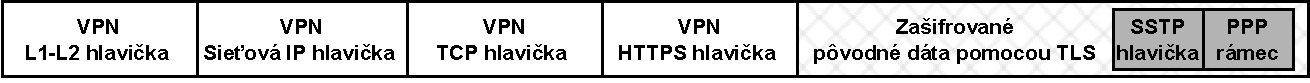
\includegraphics[width=0.3\textwidth]{figures/sstpprotocolstack}
	\caption{Proces enkapsulácie PPP rámcov pomocou protokolov naprieč SSTP protokolom}
	\label{sstpprotocolstack}
\end{figure}
Pri vytváraní SSTP segmentu dochádza k zapuzdreniu PPP rámcov pomocou HTTPS s využitím TCP protokolu s portovým číslom 443. Po úspešnom nadviazaní TCP a overení SSL/TLS spojenia dochádza k spracovaniu SSTP hlavičky. Po úspešnom odstránení sa následne získa prístup k pôvodnému PPP rámcu.   

Podobne ako tomu bolo v prípade L2TP protokolu, opísaného vyššie, tak z hľadiska premávky putujú naprieč tunelom dva druhy paketov. Vytvára a odosiela ich klient aj server. Majú špecifický formát a musia byť prenášané po bajtoch a v sieťovom poradí bajtov\footnote{z ang. \textit{network byte order}}, z ľava do prava, teda od najvýznamnejšieho bitu po najmenej významný\footnote{sieťové spracovanie dát známe aj ako z ang. \textit{Big Endian}}. Prvé 4 parametre v oboch hlavičkách sú rovnaké: 
\begin{enumerate}
	\item{\textbf{Verzia}} -- z ang. \textit{Version}, má veľkosť 8-bitov, používa sa pri komunikácií a vyjednávaní SSTP verzie, ktorá sa má použiť. Prvé 4 bity signalizujú majoritnú verziu a zvyšné minoritnú verziu. 
	\item{\textbf{Reservované}} -- z ang. \textit{Reserved}, 7 bitov nastavených na 0, rezervované pre budúce použitie, pri spracovaní sa ignorujú.
	\item{\textbf{C}} -- 1 bit, indikátor pre dátový (0) a kontrolný SSTP paket (1). 
	\item{\textbf{Dĺžka paketu}} -- z ang. \textit{LengthPacket}, 16-bitový parameter, pozostáva z:
		\begin{itemize}
			\item{\textbf{R}} -- 4 bity, pripravené na budúce použitie, nastavené na 0 a ignorované,
			\item{\textbf{Dĺžka}} -- z ang. \textit{Length}, 12 bitov, špecifikuje bajtovú veľkosť celého SSTP paketu
		\end{itemize}
\end{enumerate}
 
Rozdielnosť medzi hlavičkami vzniká v:
\begin{itemize}
	\item{\textbf{Dátové SSTP pakety}} -- z ang. \textit{SSTP Data Packets} \cite{datpak}, obsahujú 5. parameter 
		\begin{itemize}
			\item{\textbf{5. Dáta}} -- pole variabilnej dĺžky. Obsahuje zapuzdrený náklad z vyššej vrstvy.
		\end{itemize} 
	\item{\textbf{Kontrolné SSTP pakety}} -- z ang. \textit{SSTP Control Packets} \cite{conpak}, obsahuje 3 dodatočné parametre:
		\begin{itemize}
			\item{\textbf{5. Typ správy}} -- z ang. \textit{Message Type}, 16-bitové pole s SSTP správou o stave spojenia. Celkovo 9 možných správ \cite{conpak}. 
			\item{\textbf{6. Číselné atribúty}} -- z ang. \textit{Num Attributes}, 16-bitové pole, ktoré špecifikuje počet parametrov v správe
			\item{\textbf{7. Atribúty}} -- z ang. \textit{Atributes}, zoznam parametrov s variabilnou veľkosťou.
		\end{itemize}	
\end{itemize}   
 
Protokol vo všeobecnosti nepodporuje spojenie typu sieť k sieti. Primárne je orientovaný na pripojenie klienta k sieti, za účelom získania vzdialeného prístupu. To isté platí pri autentizácií. Je možné autentizovať iba používateľa, iné možnosti nie sú podporované (zariadenie, smart card, počítať,...). V prípade nestabilného spojenia, je možný vysoký výskyt straty paketov. Dôvodom je použitie TCP protokolu. 

Bezpečnosť SSTP je sprostredkovaná za pomoci HTTPS protokolu, ktorý používa SSL/TLS. Aplikované kryptografické algoritmy závisia od verzie SSL/TLS, ktorá je použitá v implementácií. TLS bol predmetom opisu v úvode práce. SSTP sa považuje za veľmi bezpečný protokol. Na druhej strane použitie robustných šifrovacích a autentizačných algoritmov, dosť spomaľuje výsledné SSTP VPN pripojenie.

Viac informácií o protokole môže čitateľ nájsť v \cite{mssstp}, odkiaľ boli aj informácie pre túto podkapitolu čerpané.  


\subsection{Ostatné populárne VPN protokoly}
Vrámci tejto práce si predstavíme ešte dvojicu veľmi populárnych VPN riešení. Koncepčne sú riešenia pri vytváraní tunelu a prenose správ podobné vyššie opísaným protokolom. Z uvedeného dôvodu protokoly len stručne charakterizujeme.
\subsubsection{OpenVPN}
OpenVPN je jeden z najznámnejšich voľne dostupných VPN tunelovacích protokolov. Vznikol v roku 2001. Dostupné ako firmvérové riešenie pre výrobcov sieťových zariadení. Pre používateľa je dostupná vo forme softvéru, ktorý je potrebné nainštalovať na cieľovú platformu. Ponúka aj grafické rozhranie. Zabezpečené spojenie naprieč internetom je sprostredkovane prostredníctvom SSL/TLS protokolu. Dokáže pracovať s dátami na L2 aj L3 vrstve v závislosti od konfigurácie. Vďaka voľnému prístupu do zdrojového kódu poskytuje jednoduché možnosti na skúmanie výsledných riešení, validáciu a prípadnú úpravu podľa potrieb konkrétneho používateľa. Protokol je napísaný v jazyku C. Bezpečnostné prvky su implementované pomocou OpenSSL knižnice. Knižnica v sebe zahŕňa funkcie potrebné na šifrovanie, autentizáciu, výmenu kľúčov a mnoho ďalšieho. Na obrázku \ref{ovpnptstrc} je znázornená výstupna štruktúra paketu po zapuzdrení. 
% TODO: \usepackage{graphicx} required
\begin{figure}[!h]
	\centering
	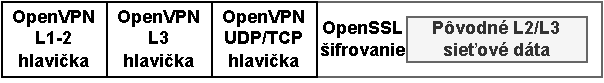
\includegraphics[width=0.5\textwidth]{figures/ovpnptstrc}
	\caption{}
	\label{ovpnptstrc}
\end{figure}

Aktuálne používa na šifrovanie AES s 256-bitovou veľkosťou kľúča. V súčasnosti sa OpenVPN považuje za najbezpečnejšiu implementáciu VPN dostupnú pre viacero platforiem. Používateľ ma možnosti vo voľbe protokolu TCP alebo UDP. Podporuje aj prácu s IPv6. OpenVPN nie je kompatabilná s ostatnými protokolmi. Je preto potrebné mať implementáciu na serveri aj klientovi. Nevýhodou je pomerne veľké, energeticky a výpočtovo náročné prevedenie.

Viac informácií o tomto komplexnom programe je možné nájsť v \cite{vpntech}, \cite{ovpn} a priamo na stránke OpenVPN\footnote{https://openvpn.net/faq/what-is-openvpn/}. Z uvedených zdrojov boli aj informácie čerpané. Zdrojový kód je dostupný napríklad na Githube\footnote{https://github.com/OpenVPN/openvpn/}. 
\subsubsection{WireGuard}

\section{Zhrnutie VPN sieti}
Jednoducha schema so vsetkym v jednom obrazku \\

 
\cite{divvpn}, \cite{ciscovpn}
https://www.vpnmentor.com/blog/different-types-of-vpns-and-when-to-use-them/
https://www.top10vpn.com/what-is-a-vpn/vpn-types/
%https://en.wikipedia.org/wiki/Virtual_private_network
%https://csrc.nist.gov/glossary/term/virtual_private_network
https://www.auvik.com/franklyit/blog/vpn-types/
https://www.geeksforgeeks.org/types-of-virtual-private-network-vpn-and-its-protocols/?ref=rp
https://www.geeksforgeeks.org/difference-between-site-to-site-vpn-and-remote-access-vpn/?ref=rp
\\
V~súčasnosti je trend, využívanie VPN na súkromné účely. Dôvodov môže byť viacero. Napríklad prístup k lokálne blokovaným doménam, anonymita v internetovom prostredí, zabezpečenie pripojenia a iné. V tomto prípade vstupujú do popredia tzv. VPN poskytovatelia (z ang. \textit{VPN Providers}). Ktorý za poplatok poskytujú výhody pripojenia cez VPN k verejnej sieti.
-- stoji za zmienku \\
https://github.com/vpnhood/VpnHood a plus v inych jazykoch 

\chapter{Ľahká kryptografia}\label{krypto}
Diplomaticky uvod do problematiky --> zdroj \\
https://csrc.nist.gov/projects/lightweight-cryptography/finalists 
https://csrc.nist.gov/CSRC/media/Projects/Lightweight-Cryptography/documents/final-lwc-submission-requirements-august2018.pdf
\section{clanok}
Cieľom kryptografických blokov je utajiť správu pri jej ceste z bodu A do B. Teda od odosielateľa (tvorcu) správy, až k jej prijímateľovi. Dôsledkom tohto úkonu dochádza k zabezpečeniu 3 hlavných úloh kryptografie:
\begin{itemize}
	\item \textbf{ochrana osobných údajov} (dôvernosť) -- z ang. \textit{Data Privacy}, 
	\item \textbf{autenticita údajov} (prišla z miesta, kde sa uvádza)  -- z ang. \textit{Data Authenticity},
	\item \textbf{integrita údajov} (nebolia upravená počas prenosu)  -- z ang. \textit{Data Integrity}.
\end{itemize}

 Prvý z uvedených bodov je najčastejšie žiadaným a známym cieľom. Odosielateľ správy zašifruje jej obsah pomocou použitia niektorého z šifrovacích algoritmov, kryptografického kľúča a následne správu odošle. Na druhej strane, prijímateľ, musí použiť komplementárny dešifrovací algoritmus s prislúchajúcim kľúčom. Ktokoľvek kto sa dostane medzi týchto komunikantov, k takto preposielanej správe, z nej nedokáže obsahovo nič zistiť, v istom časovom období. 
 
 Dôsledkom týchto faktov je jasné, že komunikanti musia mať jasne definovaný použitý algoritmus. Zároveň je nutné aby došlo k výmene kryptografických kľúčov, ktoré sú pri šifrovaní a dešifrovaní aplikované. Tým sa zabezpečí aj druhá úloha -- Autenticita dát, pretože potrebné informácie budú mať len komunikanti. 
 
 V kryptografických blokoch sú taktiež aplikované algoritmy na overenie integrity správ. Ich úlohou je potvrdiť, že do obsahu správy nebolo, počas jej transportu medzi komunikantmi, nič pridané, resp. ubrané.
 
 V súčasnosti má používateľ možnosť vybrať si zo širokej ponuky kryptografických algoritmov. Medzi najznámejší patrí \acrshort{aes} \cite{aes}, ktorý je aktuálne používaný ako štandardný kryptografický algoritmus. Detailný opis jednotlivých blokov a postupov použitých v AES-e, je obsahom rôznych vydaní. Viac informácií o problematike nájde čitateľ v \cite{levicky}, ktorá obsahuje okrem opisu AES-u aj doležité informácie, týkajúce sa kryptografických základov.

V rámci tejto práce sme sa rozhodli opísať, v súčásnosti menej známe, algoritmy: 
\begin{itemize}
	\item XOODOO \cite{tkecak}
	\item Gimli \cite{gimli}
	\item Simpira384 \cite{simpira}
\end{itemize}  
Uvedené permutácie sú použité ako kryptografické primitívum a pri následnej tvorbe ďalších kryptografickych blokov. 

\section{Kryptografický algoritmus XOODOO a variácie} 
XOODOO je sada 384-bitových kryptografických permutácií parametrizovaných počtom kôl. Funkcia kola/rundy\footnote{z ang. \textit{round}} funguje na 12 slovách\footnote{z ang. \textit{words}} po 32 bitoch. Vďaka tomu je efektívna aj na menej výkonných procesoroch nižšej triedy. Vytvoril ju tím Keccak, ktorý stojí za viacerými úspešnými kryptografickými algoritmami. Napríklad hashovacie funkcie z rodiny SHA-3 a iné -- \cite{kecsup}. XOODOO algoritmus vznikol po vytvorení tzv. Kravatte autentizačno-šifrovacieho algoritmu \cite{kravatte}, založené na Keccak-p permutácií \cite{keccakp}. Ten sa ukázal ako dostatočne rýchly na širokom spektre platforiem. Avšak nezapadá do kategórie tzv. ľahkej kryptografie \footnote{z ang. \textit{lightweight cryptography}}.

Tím Keccak vypracoval nové riešenie. Ním bol port medzi ich prvotným Keccak-p dizajnom a Gimli-ho \cite{bernstein2017gimli} permutačným algoritmom. Vo výsledku autori zlúčili lepšie realizované prvky z oboch algoritmov do jedného celku. Primárny problém samotnej Gimli permutácie bol v slabom prejave zmeny výstupu po malých zmenách vo vstupnej správe. Táto vlastnosť sa v kryptografii označuje pomocou anglického pojmu, tzv. \textit{propagation properties}\footnote{Cieľom je aby aj zmena jedného bitu na vstupe, ovplyvnila čo najviac bitov vo výstupe -- tzv. \textit{Lavínový efekt}.}. Novo-vzniknuté riešenie autori pomenovali XOODOO. Na základe rôznych variácií tohto kryptografického primitíva sa im následne podarilo vytvoriť sadu vysoko efektívnych kryptografických funkcií. 
Medzi sady, ktorých jadro tvorí XOODOO, patrí Xoodyak a Xoofff. Xoofff pozostáva zo zlúčenia Farfalle konštrukcie \cite{farfalle} so XOODOO permutáciou. 

Xoodyak ma narozdiel od Xoofff duplexovú konštrukciu \cite{duplex}. Vo výsledku máme ľahko prenosnú, všestrannú, kryptografickú knižnicu. Je vhodná do výkonovo obmedzených prostredí. Môže sa použiť pre väčšinu kryptografických funkcií, ktoré používajú symetrický kľúč. Napríklad hashovanie, šifrovanie, výpočet MAC alebo autentizované šifrovanie. O kvalite riešenia napovedá aj fakt, že sada Xoodyak je jedným z 10 finalistov v oblasti ľahkej kryptografie NIST štandardizačného procesu.
V rámci tejto kapitoly opíšeme kryptografické primitívum XOODOO a následne balík Xoodyak. Informácie o téme boli čerpané z týchto zdrojov: \cite{tkecak}, \cite{xd}, \cite{xcb}, \cite{xoodoocb}, \cite{xdupdate},\cite{xdr1}.
\subsection{XOODOO permutácia}
XOODOO je rodina permutácií, ktorá je definovaná počtom rúnd. Má klasickú iteračnú štruktúru. Teda opakovateľne sa vola rundová funkcia s aktuálnym stavom. Pre pochopenie operácií je nutné pochopiť určité označenie použité v algoritme.

Stav -- \textbf{state}, pozostáva z 3 rovnako veľkých horizontálnych rovín -- \textbf{planes}. Každá z týchto rovín obsahuje štyri paralelne 32-bitové pruhy -- \textbf{lanes}. Okrem tejto charakteristiky je možné opísať stav ako množinu 128 stĺpcov -- \textbf{columns}, pričom jeden stĺpec obsahuje 3 bity v každej rovine. Stav je teda tvorený zo stĺpcov usporiadaných v poli o rozmere 4x32. Posledná položka na opis stavu sú tzv. listy -- \textbf{sheets}. List sa skladá z 3 na sebe uložených pruhov. Uvedené pojmy sú znázornené pomocou schémy \ref{xoodooterm}, ktorá bola prebraná z \cite{xcb}.

\begin{figure}[!h]
	\centering
	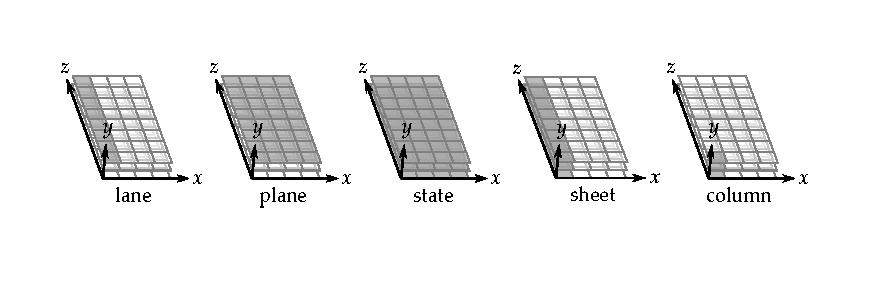
\includegraphics[width=1\textwidth]{figures/xoodooTerminology}
	\caption{Grafické znázornenie terminológie v XOODOO}
	\label{xoodooterm}
\end{figure}

Roviny majú index $y$. $y=0$ zodpovedá spodnej rovine a vrchná rovina $y=2$. Bit je označený s indexom $z$ vrámci množiny pruhov. List ich označujeme pomocou indexu $x$. Takže pozícia pruhu v stave je definovaná pomocou dvoch súradníc $(x,y)$. Konkrétny bit je možné v stave následne reprezentovať pomocou trojice súradníc $(x,y,z)$. Pri učení stĺpca sú potrebné 2 súradnice $(x,z)$. Pred spustením samotného algoritmu musí používateľ vykonať mapovanie 384-bitovej správy voči horizontálnym rovinám. Tento úkon sa realizuje pomocou vzorca \ref{index}.

\begin{equation}\label{index}
	i=z+32(x+4y)
\end{equation}

Rundová funkcia pozostáva z 5 krokov:
\begin{enumerate}
	\item miešanie vrstvy (z ang. \textit{a mixing layer $\theta$}), 
	\item posun rovín (z ang. \textit{a plane shifting $\rho_{west}$}), 
	\item pridanie rundových konštánt (z ang. \textit{the addition of round constants $\iota$}),
	\item nelineárna vrstva (z ang. \textit{a non-linear layer $\chi$}),
	\item posun rovín (z ang. \textit{an another plane shifting $\rho_{east}$}).
\end{enumerate}
Opis jednotlivých krokov je znázornený pomocou schémy \ref{xoodooalgo}, ktorá je prebratá z \cite{xcb}. Schéma opisuje jednotlivé kroky algoritmu vrátane rundových konštánt. 

  \begin{figure}[!h]
  	\centering
  	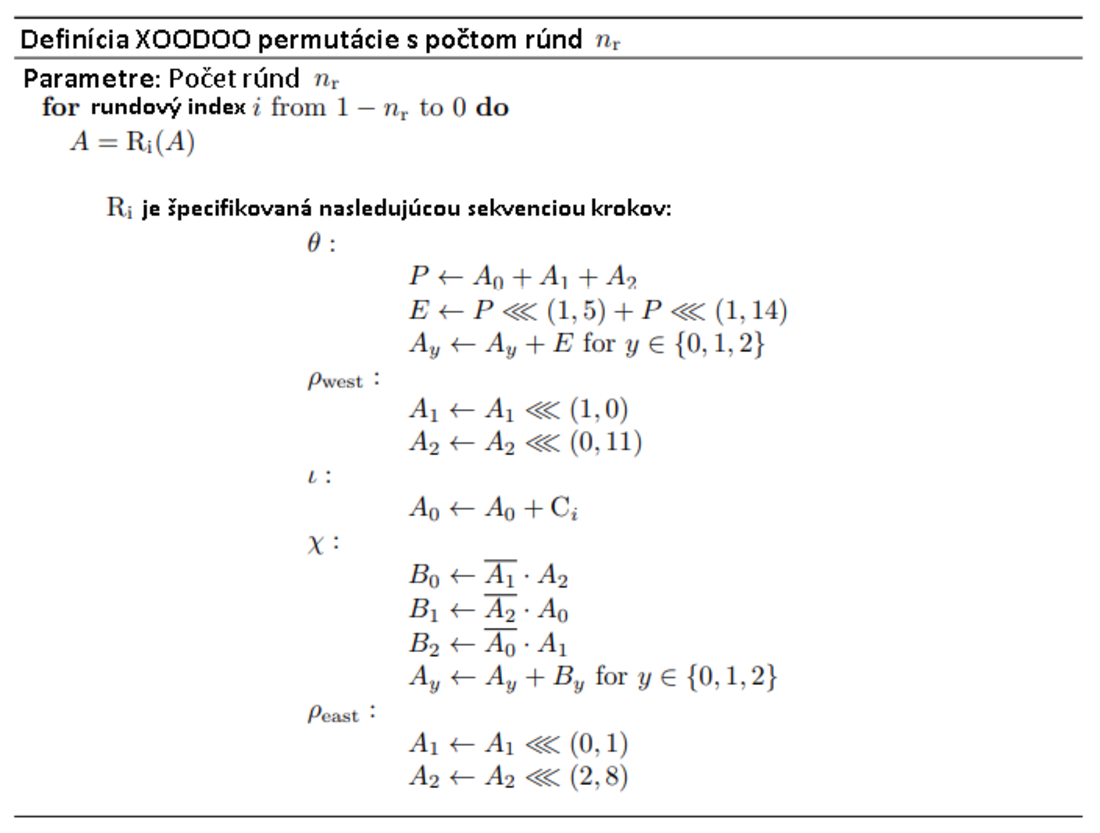
\includegraphics[width=1.1\textwidth]{figures/xoodooalgo}
  	\caption{}
  	\label{xoodooalgo}
  \end{figure}

\subsection{Xoodyak} 
Xoodyak možno považovať za všestranný kryptografický nástroj. Je vhodný pre väčšinu operácií využívajúcich symetrický kľúč. Napríklad generovanie pseudonáhodných bitov, autentizáciu, šifrovanie a iné. Tím Keccak použil pri návrhu duplexnú konštrukciu. Konkrétne variant s plným stavom a využitím kľúča. Tento dizajn označujeme ako \acrfull{fskd}. Viac o tejto konštrukcii si čitateľ môže prečítať v \cite{duplex}.
Operačný režim, v ktorom Xoodyak pracuje sa nazýva Cyklista -- z ang. \textit{Cyclist}. Tento názov získal ako opozitum k pomenovaniu režimu Motorista, ktorý je možné nájsť v Keyak schéme \cite{keyak}. Narozdiel od uvedeného balíka Keyak, nie je Xoodyak limitovaný len na autentizované šifrovanie. Je jednoduchší hlavne kvôli tomu že neobsahuje paralelné varianty.

\subsubsection{Režim Cyklista}\label{cyklista}
Režim Cyklista funguje na princípe kryptografických permutácií $f$, teda zmeny usporiadania bitov za pomoci tajného kľúča a matematických operácií. Parametrami sú veľkosti blokov $R_{hash}$, $R_{kin}$, $R_{kout}$ a veľkosť račety, resp. západky\footnote{z ang. \textit{the ratchet size}} \cite{ratchet} $\ell_{ratchet}$. Uvedený pojem sa v kryptografii používa vo forme obrazného pomenovania. Cieľom je poukázať na jednoduchý pohyb vpred, ale s ťažkým, resp. zložitejším pohybom naspäť. Dôležité je, že uvedený scenár je vyvolaný zámerným dizajnom. Šírka permutácie $b'$ je definovaná pomocou vzorca \ref{index2}. Všetky uvedené parametre sú v bajtoch. Pre označenie prázdneho slova budeme používať $\epsilon$.
\begin{equation}\label{index2}
	max(R_{hash}, R_{kin}, R_{kout}) + 2 \leq b'
\end{equation} 

Cyklista operuje v dvoch režimoch -- \textbf{hašovací a kľúčový}\footnote{z ang. \textit{hash and keyed mode}.}. 
Inicializácia prebieha pomocou príkazu \lstinline|CYCLIST(K,id,counter)|. Ak sa parameter $K$ rovná prázdnemu slovu $\epsilon$, tak potom nastane spustenie v hašovacom režime. Aktuálne nie je do implementácie zakomponovaná možnosť zmeny režimu po inicializácií. Vývojári však túto vlastnosť nevylúčili pre prípadné aktualizácie balíka.  


Dostupné funkcie závisia od režimu, v ktorom sa  Cyklista spúšťa. Medzi ne patria \lstinline|ABSORB()| a \lstinline|SQUEEZE()|. Možno ich volať v oboch režimoch, zatiaľ čo funkcie \lstinline|ENCRYPT()|, \lstinline|DECRYPT()|, \lstinline|SQUEEZEKEY()| a \lstinline|RATCHET()| sú dostupné len pre kľúčový režim. Účel každej funkcie je nasledujúci:
\begin{itemize}
	\item \lstinline|ABSORB(X)| absorbuje vstupný reťazec X,
	\item C $\gets$ \lstinline|ENCRYPT(P)| zašifruje P do C a absorbuje P,
	\item P $\gets$ \lstinline|DECRYPT(C)| dešifruje C do P a absorbuje P,
	\item Y $\gets$	\lstinline|SQUEEZE($\ell$)|  vytvára $\ell$-bajtový výstup, ktorý závisí od doteraz absorbovaných dát,
	\item Y $\gets$	\lstinline|SQUEEZEKEY($\ell$)| funguje ako \lstinline|SQUEEZE($\ell$)|, ale používa sa za účelom generovania odvodeného kľúča, 		\\ell nefunguje v listings pckg
	\item \lstinline|RATCHET()| transformuje stav na nevratný tak, aby sa zabezpečila dopredná bezpečnosť\footnote{z ang. \textit{Forward secrecy}} \cite{fsec}. 
\end{itemize}

Stav bude závisieť od postupnosti volaní funkcií a od jeho vstupných reťazcov. Presnejšie povedané, zámerom je, že akýkoľvek výstup závisí od postupnosti všetkých vstupných reťazcov a volaní, tak že akékoľvek dva nasledujúce výstupné reťazce budú výstupom rôznych domén. Napríklad volanie \lstinline|ABSORB(X)| znamená, že výstup bude závisieť od reťazca $X$. Na druhej strane \lstinline|ABSORB()| vo funkcii \lstinline|ENCRYPT(P)| vytvorí výstup závislý aj od $P$ z funkcie šifrovania. Okrem uvedených závislostí ovplyvňujú výstup aj iné dizajnové riešenia. Príkladom je minimalizácia pamäťovej stopy. Vo výsledku teda výstup závisí od počtu predchádzajúcich volaní funkcie \lstinline|SQUEEZE()| a predtým spracovaných textov pomocou funkcií \lstinline|ENCRYPT()| a \lstinline|DECRYPT()|. Viac informácií o režime je dostupných v kapitole 7.2, publikácie \cite{xcb}. 

\subsubsection{Definícia a bezpečnosť}
Xoodyak je definovaný pomocou operatívneho režimu Cyklista nasledovne:
\begin{equation}
	CYCLIST[f,R_{hash},R_{kin},R_{kout},\ell_{ratchet}]
\end{equation} 
Kde jednotlivé parametre majú veľkosti:
\begin{enumerate}
	\item $f$ -- permutácia XOODOO so šírkou 48 bajtov (384 bitov),
	\item $R_{hash}$ -- 16 bajtov,
	\item $R_{kin}$ -- 44 bajtov,
	\item $R_{kout}$ -- 24 bajtov,
	\item $\ell_{ratchet}$ -- 16 bajtov.  
\end{enumerate}
Takto definované parametre algoritmu dokážu poskytnúť 128-bitovú bezpečnosť v oboch režimoch Cyklistu. Samozrejmosťou je, že v prípade kľúčového režimu, musí byť veľkosť kľúča rovná alebo väčšia ako 128 bitov. Viac informácií o kryptografickej bezpečnosti algoritmov je možné nájsť v \cite{sec}.

Viac informácií o bezpečnosti Xoodyak-a je možné nájsť v \cite{xcb, 7.3}, odkiaľ boli informácie čerpané.

\subsection{Možnosti použitia Xoodyak algoritmu}
Obsahom tejto podkapitoly sú uvedené postupy ako a za akých okolností je daný balík možné použiť. 
\subsubsection{Použitie hašovacieho režimu}
Xoodyak sa dá aplikovať ako hašovacia funkcia.
\subsubsection{Použitie kľúčového režimu}
